\subsection{Self-Consistency and Phase Transitions}

In order to solve the self-consistent equation, we can analyze it graphically by plotting the function \(m\) on the left-hand side and the function \(\tanh\left( \beta h_{eff} \right)\) on the right-hand side as functions of \(m\). The points where these two functions intersect correspond to the solutions of the self-consistent equation. By varying the temperature \(T\) and the external field \(h\), we can observe how the number and nature of the solutions change, which provides insights into the phase transition and critical behavior of the system. Let us start from the case \(h=0\):\TODO{fix the plot}
\begin{figure}[H]
    \begin{minipage}{0.6\textwidth}
        \centering
        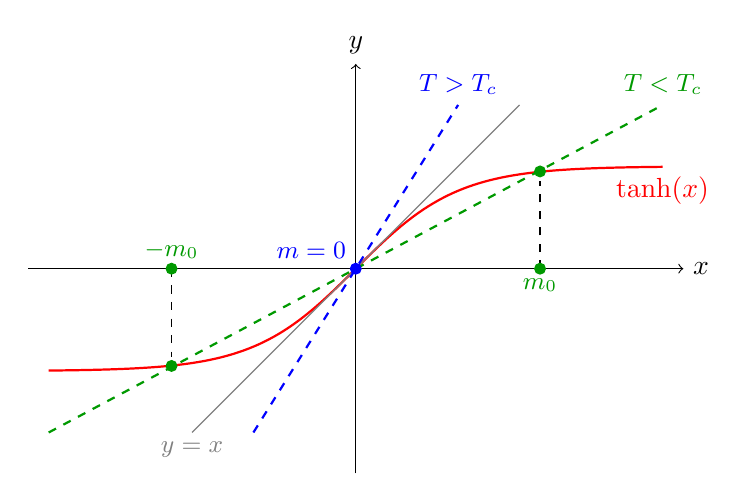
\begin{tikzpicture}[scale=1.3]

            \draw[->] (-3.2,0) -- (3.2,0) node[right] {$x$};
            \draw[->] (0,-2) -- (0,2) node[above] {$y$};

            \draw[thick,red,domain=-3:3,samples=200]
            plot (\x,{tanh(\x)}) node[below] {$\tanh(x)$};

            \draw[gray] (1.6,1.6) -- (-1.6,-1.6)
            node[below] {\small $y=x$};

            \draw[blue,thick,dashed] (-1,-1.6) -- (1,1.6)
            node[above] {\small $T>T_c$};

            \draw[green!60!black,thick,dashed] (-3,-1.6) -- (3,1.6)
            node[above] {\small $T<T_c$};

            \draw[dashed] (1.8,0) -- (1.8,0.859);
            \draw[dashed] (-1.8,0) -- (-1.8,-0.859);

            \filldraw[green!60!black] (1.8,0) circle (1.5pt) node[below] {\small $m_0$};
            \filldraw[green!60!black] (-1.8,-0) circle (1.5pt) node[above] {\small $-m_0$};
            \filldraw[green!60!black] (1.8,0.95) circle (1.5pt);
            \filldraw[green!60!black] (-1.8,-0.95) circle (1.5pt);

            \filldraw[blue] (0,0) circle (1.5pt) node[above left] {\small $m=0$};
        \end{tikzpicture}
    \end{minipage}
    \hfill
    \begin{minipage}{0.35\textwidth}
        The graphical solution shows that for \(T > T_c\) the only intersection is at the origin, yielding \(m=0\): this corresponds to the \textbf{paramagnetic phase}. For \(T < T_c\), instead, the line intersects the curve at two symmetric non-zero points, corresponding to two stable ordered states with opposite magnetization: this is the \textbf{ferromagnetic phase}.
    \end{minipage}
\end{figure}
\begin{itemize}
    \item For \(T > T_c\), there is only one solution at \(m = 0\), which corresponds to the paramagnetic phase where the spins are disordered and there is no net magnetization.
    \item For \(T < T_c\), there are three solutions: one at \(m = 0\) and two symmetric solutions at \(m = \pm m^*\), which correspond to the ferromagnetic phase where the spins are aligned and there is a non-zero magnetization. The solution at \(m = 0\) becomes unstable (not a minimum) in this regime, while the two symmetric solutions represent the stable ordered phases.
    \item At \(T = T_c\), the solution at \(m = 0\) becomes marginally stable, and the system undergoes a second-order phase transition from the paramagnetic phase to the ferromagnetic phase. The magnetization \(m\) changes continuously across the transition, and there is no latent heat associated with the transition.
\end{itemize}
The critical temperature \(T_c\) is determined by the condition that the slope of the \(\tanh\) function at \(m = 0\) equals 1, which gives
\[
    \beta_c J z = 1 \quad \Rightarrow \quad T_c = \frac{J z}{k_B},
\]
where \(k_B\) is the Boltzmann constant. Thus the condition on the critical temperature can be expressed as \(\beta_c J z = 1\).

We can now study the beaviour of the magnetization as a function of temperature.\TODO{add plot of m vs T}
As we decreas the temperature \(T\) below \(T_c\), the magnetization \(m\) increases continuously from zero, indicating the onset of ferromagnetic order. We got two symmetric solutions for the magnetization, which correspond to the two possible orientations of the spins in the ferromagnetic phase. The magnetization \(m\) serves as an order parameter that characterizes the phase transition: it is zero in the paramagnetic phase and becomes non-zero in the ferromagnetic phase, indicating the spontaneous breaking of symmetry.

We can obtain the plot of the free energy as a function of the magnetization \(m\) for different temperatures to visualize the phase transition. For \(T > T_c\), the free energy has a single minimum at \(m = 0\), corresponding to the stable paramagnetic phase. As we decrease the temperature below \(T_c\), the free energy develops two symmetric minima at \(m = \pm m^*\), corresponding to the stable ferromagnetic phases, while the minimum at \(m = 0\) becomes a local maximum, indicating that it is no longer a stable solution. This can be seen studying the expression for the free energy density \(f(m)\) that we derived earlier as \(h=0\):
\[
    f(m) = \dots
\]
and we get then two different expressions for \(T > T_c\) and \(T < T_c\):\TODO{add plot of f(m) vs m for different T}
\begin{itemize}
    \item For \(T > T_c\), the free energy has a single minimum at \(m = 0\), which corresponds to the stable paramagnetic phase: we have a parabula with a minimum at the origin, which is the only stable solution in this regime.
    \item For \(T < T_c\), the free energy develops two symmetric minima at \(m = \pm m^*\), which correspond to the stable ferromagnetic phases, while the minimum at \(m = 0\) becomes a local maximum, indicating that it is no longer a stable solution: we have a double-well potential with two minima at \(m = \pm m^*\) and a local maximum at \(m = 0\). As the temperature decreases further below \(T_c\), the minima at \(m = \pm m^*\) become deeper, indicating that the ferromagnetic phases become more stable.
\end{itemize}
If we were to plot the free energy as a function of the magnetization \(m\) for different temperatures, we would see how the shape of the free energy changes across the phase transition, with the emergence of two minima below \(T_c\) and the disappearance of the minimum at \(m = 0\). This visualization helps to understand the nature of the phase transition and the role of the magnetization as an order parameter.

If we now imagine to ``turn on'' the external magnetic field \(h\), we would see that the symmetry between the two minima at \(m = \pm m^*\) is broken, and one of the minima becomes deeper than the other, depending on the sign of \(h\). The easier way is to consider an external field which is positive but very small in comparison to the coupling constant \(J\), so that we can treat it as a perturbation.\TODO{add plot of f(m) vs m for different h}
\begin{itemize}
    \item For \(h > 0\), the minimum at \(m = +m^*\) becomes deeper than the minimum at \(m = -m^*\), indicating that the ferromagnetic phase with positive magnetization is more stable than the one with negative magnetization. The system will preferentially align its spins in the direction of the external field, leading to a net positive magnetization.
    \item For \(h < 0\), the minimum at \(m = -m^*\) becomes deeper than the minimum at \(m = +m^*\), indicating that the ferromagnetic phase with negative magnetization is more stable than the one with positive magnetization. The system will preferentially align its spins in the opposite direction of the external field, leading to a net negative magnetization.
\end{itemize}
This means that the external magnetic field \(h\) breaks the \(\mathbb{Z}_2\) symmetry between the two ferromagnetic phases and selects one of them as the stable phase, depending on the sign of \(h\). This is a manifestation of the fact that the external field acts as a symmetry-breaking field, which can influence the behavior of the system near the critical point and affect the nature of the phase transition, especially in the presence of a small external field where the system can exhibit critical behavior and scaling properties.

\begin{remark}[On Symmetries and Spontaneous Symmetry Breaking]
    A symmetry of a system is a transformation that leaves the Hamiltonian (and so the physical properties and evolution of the system) invariant.

    In the case of the Ising model with \(h=0\), there is a \(\mathbb{Z}_2\) symmetry corresponding to the transformation \(s_i \to -s_i\) for all spins, which leaves the Hamiltonian unchanged:
    \[
        H(\{s_1, s_2, \ldots, s_n\}) = H(\{-s_1, -s_2, \ldots, -s_n\}).
    \]
    When we flip all spins, is like changing the sign of the magnetization \(m\), but the Hamiltonian remains the same; in the graph of the free energy, this corresponds to the symmetry of the double-well potential around \(m=0\). This symmetry is a fundamental property of the system and plays a crucial role in determining the nature of the phase transition and the behavior of the system near the critical point.

    This symmetry is \textbf{spontaneously broken} as \(T > T_c\), since ...

    Once the system is in one of the two ferromagnetic phases (with \(m = +m^*\) or \(m = -m^*\)), we could expect the system to be able to transition between these two phases by flipping all the spins, since the states are completely symmetric: same energy, entropy etc. However, in the thermodynamic limit \(N \to \infty\), the system becomes trapped in one of the two minima of the free energy, and it cannot transition to the other minimum due to the presence of an infinite energy barrier between them: the transition probability between the two minima approches zero as a power law, and the system remains in one of the two ferromagnetic phases.
\end{remark}

\subsection{Critical Exponents}

The mean field theory allows us to compute the critical exponents that characterize the behavior of the system near the critical point. By analyzing the self-consistent equation for the magnetization and the free energy, we can derive expressions for the critical exponents \(\alpha\), \(\beta\), \(\gamma\), and \(\delta\) in terms of the parameters of the model. The mean field theory predicts specific values for these critical exponents, which can be compared to experimental results and more sophisticated theoretical approaches to understand the limitations and applicability of mean field theory in describing critical phenomena.

We start from the analysis of the \textbf{free energy} \(f(m)\) and the magnetization \(m\) as a function of temperature \(T\) near the critical point \(T_c\). We can expand the the free energy in a Taylor series around \(m = 0\) to analyze the behavior of the system near the critical point. The expansion takes the form:\TODO{correct the expansion}
\[
    f(m) \sim T \left[ \frac{m^2}{2}\left(1-\frac{T}{T_c}\right) + \frac{m^4}{12} T_c^3 + O(m^6) \right],
\]
where the interesting feature is that the coefficient of the \(m^2\) term changes sign at \(T = T_c\), which indicates the onset of the phase transition. We can now find an analytic expression for the derivative of the free energy with respect to \(m\) and set it to zero to find the equilibrium magnetization \(m\) as a function of temperature \(T\):
\[
    \frac{\partial f}{\partial m} \propto m(T - T_c) + B m^3 + O(m^5) = 0, \quad B \sim O(1) > 0,
\]
which can be solved to find the behavior of the magnetization near the critical point. For \(T > T_c\), the only solution is \(m = 0\), while for \(T < T_c\), we have two symmetric solutions given by
\[
    m = \pm \sqrt{\frac{T_c - T}{B}} \sim (T_c - T)^{1/2},
\]
which indicates that the magnetization \(m\) behaves as a power law near the critical point with a critical exponent
\[
    m \propto (T_c - T)^{\beta}, \quad \beta = \frac{1}{2}.
\]
This critical exponent \(\beta\) characterizes the behavior of the magnetization as the system approaches the critical temperature from below, and it is a key quantity in understanding the nature of the phase transition.

We can now analyze the behavior of the \textbf{magnetic susceptibility} \(\chi\) near the critical point. The magnetic susceptibility is defined as the derivative of the magnetization with respect to the external magnetic field \(h\) at \(h = 0\):
\[
    \chi = \left. N\frac{\partial m}{\partial h} \right|_{h=0}.
\]
Recovering the expression for the magnetization
\[
    m = \tanh\left( \beta (h + J z m) \right),
\]
we know that near the critical point (approached from above)\(T_c\), the magnetization \(m\) is small, so we can expand the \(\tanh\) function to first order in \(m\):
\[
    m \approx \beta (h + J z m).
\]
Thus the magnetic susceptibility can be computed as
\[
    \chi = \frac{N \beta}{1 - \beta J z},
\]
which diverges as \(T\) approaches \(T_c\) from above, since \(\beta J z = 1\) at \(T = T_c\). The critical exponent \(\gamma\) characterizes the divergence of the magnetic susceptibility near the critical point, and it can be defined as
\[
    \chi \propto |T - T_c|^{-\gamma}, \quad \gamma = 1.
\]

These critical exponents helps us to understand the behavior of the system near the critical point and to classify the universality class of the phase transition. Usually when quantities diverge at the critical point, we can characterize their behavior by a power law with a critical exponent, which provides insights into the nature of the fluctuations and correlations in the system as it undergoes a phase transition. Indeed in an experiments, we can measure also \textbf{finite size effect}: all of our computations are true in the thermodynamic limit \(N \to \infty\), but in a real experiment we have a finite number of particles, so we can observe how the critical behavior is affected by the finite size of the system, which can lead to rounding and shifting of the critical point, as well as modifications to the scaling behavior of physical quantities near the transition. All of these is heavily connected to the concept of \textbf{correlation length}, which is a measure of how far correlations between particles extend in the system, and it diverges at the critical point, leading to long-range correlations and critical fluctuations that dominate the behavior of the system near the transition.

How can we concile the mean field predictions for the critical exponents with experimental results? The mean field theory provides is just an approximation, and it is known to give incorrect predictions for the critical exponents in low-dimensional systems (e.g., 2D and 3D), where fluctuations play a significant role (speaking about the Ising model). In higher dimensions (e.g., 4D and above), the mean field theory becomes more accurate, and the critical exponents predicted by mean field theory are closer to experimental results. For Ising
\begin{itemize}
    \item In 1D, the Ising model does not exhibit a phase transition at finite temperature, and the critical exponents are not defined in the usual sense. The mean field theory incorrectly predicts a phase transition in 1D, which is a clear indication of its limitations in low-dimensionality.
    \item In 2D, the exact solution of the Ising model gives \(\beta = 1/8\) and \(\gamma = 7/4\), which are different from the mean field predictions.
    \item In 3D, numerical simulations and experiments suggest that \(\beta \approx 0.326\) and \(\gamma \approx 1.237\), which again differ from the mean field values.
    \item In 4D and above, the critical exponents approach the mean field values of \(\beta = 1/2\) and \(\gamma = 1\).
\end{itemize}
Here we can see that the mean field theory provides a qualitative understanding of the phase transition and critical behavior, but it fails to capture the correct critical exponents in low-dimensional systems due to the neglect of fluctuations, which are crucial in determining the behavior near the critical point. More sophisticated approaches, such as renormalization group theory, are needed to accurately describe critical phenomena and compute critical exponents in low-dimensional systems.

We will solve the Ising model in 1D in the next section, and we will give some arguments about the behavior of the model in 2D, which will allow us to understand better the limitations of mean field theory and the importance of fluctuations in low-dimensional systems.

\subsection{1D-Ising Model}

The hamiltonian of the 1D Ising model is given by
\[
    H = -J \sum_{i=1}^{N} s_i s_{i+1} - h \sum_{i=1}^{N} s_i,
\]
where we have periodic boundary conditions \(s_{N+1} = s_1\). The partition function depends upon the temperature \(T\), the external magnetic field \(h\) and the number of spins \(N\), and it can be written as
\[
    Z_N(\beta, h) = \sum_{\{s_i\}} e^{-\beta H(\{s_i\})}.
\]
It is important since we can derive an expression for the ensemble average of the magnetization per site as a function of the partition function:
\[
    \mathbb{E}_c \left[ \frac{1}{N} \sum_{i=1}^{N} s_i \right] = - \frac{1}{N\beta} \frac{\partial \log Z_N}{\partial h}.
\]
If we manipulate the expression of the hamiltonian, to express two symmetric sums, we get
\[
    H = -J \sum_{i=1}^{N} s_i s_{i+1} - \frac{h}{2} \sum_{i=1}^{N} s_i s_{i+1}
\]
\[
    Z = \sum_{\{s_i\}} \prod_{i=1}^{N} (e^{\beta J s_i s_{i+1} + \frac{\beta h}{2} s_i s_{i+1}})\dots
\]

Now we can introduce the \textbf{transfer matrix} \(T\), which is a \(2 \times 2\) matrix that encodes the interactions between neighboring spins and the effect of the external magnetic field. The transfer matrix is defined as
\[
    T_{s_i, s_{i+1}} = e^{\beta J s_i s_{i+1} + \frac{\beta h}{2} (s_i + s_{i+1})},
\]
where \(s_i\) and \(s_{i+1}\) can take values of \(\pm 1\). The partition function can then be expressed as a product of transfer matrices:
\[
    Z = \sum_{\{s_i\}} T_{s_1, s_2} T_{s_2, s_3} \cdots T_{s_N, s_1} = \text{Tr}(T^N),
\]
where the trace is taken over the possible spin states. The transfer matrix method allows us to compute the partition function and other thermodynamic quantities by diagonalizing the transfer matrix and finding its eigenvalues. The largest eigenvalue of the transfer matrix dominates the behavior of the partition function in the thermodynamic limit, and it can be used to derive expressions for the free energy, magnetization, and other physical quantities of interest. This method is particularly powerful for solving one-dimensional models like the 1D Ising model, where it provides an exact solution for the partition function and allows us to analyze the behavior of the system at different temperatures and external fields.



\subsubsection{Diagonalization and Phase Transitions}

Expressing the partition function in terms of the transfer matrix, we can notice how the computational complexity of the problem is reduced from summing over \(2^N\) configurations to diagonalizing a \(2 \times 2\) matrix multiplied \(N\) times with itself, which is a much more tractable problem. The eigenvalues of the transfer matrix can be computed explicitly, and they determine the thermodynamic properties of the system. We can write the transfer matrix explicitly as
\[
    T = \begin{pmatrix}
        e^{\beta J + \beta h} & e^{-\beta J}          \\
        e^{-\beta J}          & e^{\beta J - \beta h}
    \end{pmatrix},
\]
with the idea of diagonalizing this matrix to find its eigenvalues \(\lambda_1\) and \(\lambda_2\). Let us note that \(T = T^{\dagger}\), thus we know there exist an orthogonal matrix \(O = O^T\) such that \(T = O D O^{T}\), where \(D\) is a diagonal matrix containing the eigenvalues of \(T\). The diagonal maatrix \(D\) can be expressed as
\[
    D = \begin{pmatrix}
        \lambda_+ & 0         \\
        0         & \lambda_-
    \end{pmatrix},
\]
and we can compute the the \(N\)th power of the transfer matrix as
\[
    T^N = (ODO^T)^N = (ODO^T)(ODO^T)\cdots(ODO^T) = O D^N O^T,
\]
where we have used the fact that \(O^T O = I\) to simplify the expression. The partition function can then be expressed as
\[
    Z = \text{Tr}(T^N) = \text{Tr}(O D^N O^T) = \text{Tr}(D^N) = \lambda_+^N + \lambda_-^N,
\]
where \(\lambda_+\) and \(\lambda_-\) are the eigenvalues of the transfer matrix \(T\) and we have used the cyclic property of the trace.

Now we can also compute the determinant of the transfer matrix, which is given by
\[
    \det(T) = \lambda_+ \lambda_- = e^{2\beta J} - e^{-2\beta J} = 2 \sinh(2\beta J),
\]
while for the trace we had
\[
    \text{Tr}(T) = \lambda_+ + \lambda_- = e^{\beta J + \beta h} + e^{\beta J - \beta h} + 2 e^{-\beta J} = 2 e^{\beta J} \cosh(\beta h) + 2 e^{-\beta J}.
\]
The eigenvalues of the transfer matrix can be computed using the characteristic polynomial, which is given by
\[
    x^2 - \text{Tr}(T) x + \det(T) = 0,
\]
which, inserting the expressions for the trace and determinant, can be rewritten as
\[
    \dots
\]
and in the end we get the eigenvalues as
\[
    \lambda_{\pm} = e^{\beta J} \left(\cosh(\beta h) \pm \sqrt{\sinh^2(\beta h) + e^{-4\beta J}}\right),
\]
which gives
\[
    \vert \frac{\lambda_-}{\lambda_+} \vert <1 , \quad \vert \frac{\lambda_-}{\lambda_+} \vert^N \ll 1.
\]
thus we can write the partition function in the thermodynamic limit as
\[
    Z = \lambda_+^N + \lambda_-^N = \lambda_+^N \left(1 + \left(\frac{\lambda_-}{\lambda_+}\right)^N\right) \approx \lambda_+^N,
\]
which allows us to compute the free energy per site as
\[
    f = -\frac{1}{\beta} \lim_{N \to \infty} \frac{1}{N} \log Z,
\]
where \(f = \lim_{N \to \infty} \frac{F}{N}\); thus we have
\[
    f = -\frac{1}{\beta} \log \lambda_+ = -J - \frac{1}{\beta} \log\left( \cosh(\beta h) + \sqrt{\sinh^2(\beta h) + e^{-4\beta J}} \right).
\]
from this we can understand that there are no singularities in the free energy as a function of temperature \(T\) and external field \(h\), which indicates that there is no phase transition in the 1D Ising model at finite temperature. This is consistent with the known result that the 1D Ising model does not exhibit a phase transition at finite temperature, and it highlights the importance of dimensionality and fluctuations in determining the behavior of the system near critical points.

Let us now compute the magnetization per site as a function of temperature \(T\) and external field \(h\). We can use the expression for the partition function to compute the magnetization as
\[
    \mathbb{E}_{c}\left[s_i\right] = m = -\frac{1}{N} \frac{\partial}{\partial h} \log Z = -\frac{1}{\beta} \frac{\partial}{\partial h} (\frac{F}{N}).
\]
Inserting the expression for the free energy per site, we get
\[
    m = \frac{\sinh(\beta h)}{\sqrt{\sinh^2(\beta h) + e^{-4\beta J}}}.
\]
This expression shows that the magnetization \(m\) is a smooth function of temperature \(T\) and external field \(h\), and it does not exhibit any singularities or discontinuities, which is consistent with the absence of a phase transition in the 1D Ising model at finite temperature.

\TODO{add plot of m vs h for different T.}

As \(T\) increases, the curve becomes more steep, but it never exihibit a discontinuity or a singularity, which confirms that there is no phase transition in the 1D Ising model at finite temperature. Only in the limit \(T \to 0\) we have a discontinuity in the magnetization at \(h = 0\), where the system transitions from a fully magnetized state with \(m = +1\) for \(h > 0\) to a fully magnetized state with \(m = -1\) for \(h < 0\):
\[
    \lim_{T \to 0} m(T,h) = \text{sgn}(\sinh(\beta h)) = \text{sgn}(h).
\]

We could repeat the computation for \(\chi\) the magnetic susceptibility, which is given by
\[
    \chi = \frac{\partial}{\partial h} m(T,h) = \dots
\]
and it can be shown that \(\chi\) does not diverge at any finite temperature, which is consistent with the absence of a phase transition in the 1D Ising model at finite temperature. Only in the limit \(T \to 0\) we have a divergence in the magnetic susceptibility at \(h = 0\), which indicates a critical point at zero temperature.

The euristic derivation of mean field theory has to have some assumptions which do not hold at low dimensions, and this is the reason why it fails to capture the correct critical behavior in 1D and 2D systems. Only in higher dimensions, where fluctuations are less important, the mean field theory provides a more accurate description of the critical behavior and the critical exponents.

The exact solution of the 1D Ising model using the transfer matrix method allows us to understand the limitations of mean field theory and the importance of fluctuations in determining the behavior of the system near critical points.

\subsubsection{Two Point Correlation Function}

It is now time to compute the two-point correlation function for the 1D Ising model: the correlation function is defined as
\[
    \mathbb{E}_{c}\left[ s_i s_{i+r} \right] = \frac{1}{Z} \sum_{\{s_k\}} s_i s_{i+r} e^{-\beta H(\{s_k\})},
\]
which can become a connected correlation function if we subtract the product of the magnetizations:
\[
    \mathbb{E}_{c}\left[ s_i s_{i+r} \right] - \mathbb{E}_{c}\left[ s_i \right] \mathbb{E}_{c}\left[ s_{i+r} \right] = \frac{1}{Z} \sum_{\{s_k\}} s_i s_{i+r} e^{-\beta H(\{s_k\})} - m^2.
\]
To compute the correlation function, we can use the transfer matrix method again. We can express the correlation function in terms of the transfer matrix as follows:
\[
    \mathbb{E}_{c}\left[ s_i s_{i+r} \right] = \frac{1}{Z} \sum_{\alpha_1=1}^2 \sum_{\alpha_2=1}^2 \dots \sum_{\alpha_N=1}^2 \sigma_{\alpha_j} \sigma_{\alpha_{j+r}} T_{\alpha_1, \alpha_2} T_{\alpha_2, \alpha_3} \cdots T_{\alpha_N, \alpha_1},
\]
where \(\sigma_{\alpha_j}\) is the spin value corresponding to the state \(\alpha_j\) (i.e., \(\sigma_1 = +1\) and \(\sigma_2 = -1\)). We can rewrite this expression in a more compact form using matrix notation. Let us define a diagonal matrix \(D\) such that
\[
    D = \begin{pmatrix}
        1 & 0  \\
        0 & -1
    \end{pmatrix}, \text{ and } D_{\alpha,\beta} = \delta_{\alpha,\beta} \cdot \sigma_{\alpha},
\]
meaning that \(D\) is a diagonal matrix with entries corresponding to the spin values. Then we can express the correlation function as
\[
    \mathbb{E}_{c}\left[ s_j s_{j+r} \right] = \frac{1}{Z} \sum_{\alpha_1=1}^2 \sum_{\alpha_2=1}^2 \dots \sum_{\alpha_N=1}^2 T_{\alpha_1, \alpha_2} T_{\alpha_2, \alpha_3} \cdots T_{\alpha_{j-1}, \alpha_j} D_{\alpha_j, \beta_1} T_{\beta_1, \alpha_{j+1}} \cdots T_{\alpha_{j+r-1}, \alpha_{j+r}} D_{\alpha_{j+r}, \beta_2} T_{\beta_2, \alpha_{j+r+1}} \cdots T_{\alpha_N, \alpha_1},
\]
where we have inserted the diagonal matrices \(D\) at the positions corresponding to the spins \(s_j\) and \(s_{j+r}\). This expression can be further simplified by recognizing that the sums over the indices \(\alpha_k\) correspond to matrix multiplications, and we can express
\[
    \mathbb{E}_{c}\left[ s_j s_{j+r} \right] = \frac{1}{Z} \text{Tr}(T^{j-1} D T^{r} D T^{N-r+1-j}),
\]
where we have used the cyclic property of the trace to rearrange the order of the matrices. This expression allows us to compute the two-point correlation function in terms of the transfer matrix and the diagonal matrix \(D\), which encodes the spin values. By diagonalizing the transfer matrix with a unitary matrix \(U\):
\[
    T = U \begin{pmatrix}
        \lambda_+ & 0         \\
        0         & \lambda_-
    \end{pmatrix} U^{\dagger},
\]
where \(U\) can be computed explicitly, we can express the correlation function in terms of the eigenvalues and eigenvectors of the transfer matrix, which allows us to analyze its behavior as a function of the distance \(r\) and the temperature \(T\). Let us focus on the case without external field: the unitary transformation becomes
\[
    \dots
\]
and so we can write the transfer matrix in the diagonal basis as
\[
    \dots
\]
Now putting everything together, we can express the correlation function as
\[
    \begin{aligned}
        \dots
    \end{aligned}
\]
In the end we find a close analytical form for the correlation function, which can be expressed as
\[
    \mathbb{E}_{c}\left[ s_j s_{j+r} \right]_{h=0} = \frac{\lambda_+^{N-r}\lambda_-^r + \lambda_-^{N-r}\lambda_+^r}{\lambda_+^N + \lambda_-^N},
\]
and again if we use tha fact that \(\vert \frac{\lambda_-}{\lambda_+} \vert < 1\), we can simplify this expression in the thermodynamic limit as
\[
    \mathbb{E}_{c}\left[ s_j s_{j+r} \right]_{h=0} =\dots \sim e^{-\tfrac{r}{\xi}},
\]
effectively defining the correlation length \(\xi\) as
\[
    \xi^{-1} = \log(\frac{\lambda_+}{\lambda_-}) > 0,
\]
which is a measure of how far correlations between spins extend in the system.
Now considering the absence of an external field, we can express the eigenvalues of the transfer matrix as
...

and in the end we get the correlation length in the \(T \to 0\) limit without external field as
\[
    \xi \sim e^{2\beta J},
\]
so that it diveres exponentially as \(T \to 0\), which indicates that the system exhibits long-range correlations at low temperatures, and it confirms the presence of a critical point at zero temperature in the 1D Ising model. This behavior of the correlation length is consistent with the absence of a phase transition at finite temperature, as the correlation length remains finite for all \(T > 0\) and only diverges as \(T \to 0\).

The correlation lenght correspond to the distance after which we can consider the spins as independent, since the correlation function decays exponentially with distance \(r\) as \(e^{-r/\xi}\). As the temperature approaches zero, the correlation length diverges, indicating that the spins become correlated over longer distances, which is a signature of critical behavior at zero temperature. This analysis of the two-point correlation function and the correlation length provides insights into the nature of correlations in the 1D Ising model and helps to understand the absence of a phase transition at finite temperature. But since this divergence occur at \(T=0\) then everything is in accord to the fact that there is no phase transition at finite temperature, and the critical point is located at zero temperature.


\subsection{2D-Ising Model}

We will not solve exactly the 2D Ising model, but we will give some arguments about its behavior and the nature of the phase transition it exhibits, and then in the end we will present the proof of the existence of a phase transition in the 2D Ising model at finite temperature, which is a non-trivial result that highlights the importance of dimensionality and fluctuations in determining the behavior of the system near critical points.

\subsubsection{Phase Transition - Euristic}

Consider the 2D Ising model on a square lattice, where each spin interacts with its four nearest neighbors. Take the limit for a very low temperature \(T \to 0\), and suppose that there is a region in the first 1D raw where the system is in a fully magnetized state, with all \(l\) spins aligned (e.g., \(m = +1\)). We want to ask ourselves if this state is stable against the formation of a droplet of flipped spins (e.g., \(m = -1\)) of size \(l \times l\). The energy cost of creating such a droplet can be estimated as follows:
\begin{itemize}
    \item Case A: \(\uparrow\,\uparrow\,\dots \,\uparrow \), where we have a single domain wall of length \(l\) separating the two regions of opposite magnetization. The energy cost of creating this domain wall is proportional to its length, which gives
          \[
              E = - J l,
          \]
          where \(J\) is the coupling constant. The energy cost is negative, which means that it is energetically favorable to create such a droplet, and the system will tend to form domains of flipped spins, leading to a disordered state with zero magnetization.
    \item Case B: \(\uparrow\,\dots \,\uparrow \,\downarrow\,\dots \,\downarrow \), where we have two domain walls of length \(l\) separating the three regions of magnetization. The energy cost of creating these two domain walls is proportional to their total length, which gives
          \[
              E = - J l + 2 J l = J l,
          \]
          where the first term corresponds to the energy cost of creating the first domain wall, and the second term corresponds to the energy cost of creating the second domain wall. The energy cost is positive, which means that it is energetically unfavorable to create such a droplet.
\end{itemize}

\begin{remark}[entropy of domains]
    ...
\end{remark}

If we now compute the free energy cost of creating such a droplet, we need to take into account both the energy cost and the entropy gain associated with the formation of the droplet. The free energy cost can be expressed as
\[
    F_B - F_A = \Delta E - T \Delta S = 2 J l - T k_B \log(l-1),
\]
since the energy cost of creating the droplet in case B is \(2 J l\) and the entropy gain is proportional to the logarithm of the number of ways to arrange the droplet, which is approximately \(\log(l-1)\). As \(l\) increases, the energy cost dominates over the entropy gain, and the free energy cost becomes positive, which means that it is energetically unfavorable to create such a droplet. This indicates that the system will tend to remain in a magnetized state with non-zero magnetization, and it suggests that there is a phase transition at a finite temperature \(T_c\) below which the system exhibits spontaneous magnetization.

This argument provides an intuitive understanding of why the 2D Ising model exhibits a phase transition at finite temperature, and it highlights the importance of dimensionality and fluctuations in determining the behavior of the system near critical points.

It seems that breaking a domain wall is energetically unfavorable, but there is a maximum value of \(l\) for which the entropy does not make unfavorable the creation of the droplet, and this maximum value of \(l\) can be estimated by setting the free energy cost to zero:
\[
    \Delta F = 0 \implies 2 J l - T k_B \log(l-1) = 0 \implies l \sim e^{\frac{2 J}{T k_B}} = \xi,
\]
which indicates that there is a characteristic length scale \(l\) above which the domain wall are not favorable anymore, and this length scale can be identified with the correlation length \(\xi\) of the system. As the temperature approaches the critical temperature \(T_c\) from below, the correlation length diverges, indicating that the system exhibits long-range correlations and critical behavior at the phase transition.

Euristic arguments in statistical physics can provide valuable insights into the behavior of complex systems and help to understand the underlying mechanisms driving phase transitions and critical phenomena. Sometimes, when a problem is mathematically intractable, we can use physical intuition and qualitative reasoning to make predictions about the behavior of the system, which can then be used to address the problem in new ways and in the end find the analutical solution.

\subsubsection{Peierls's argument - Euristic}

Let us compare the free energy of the two configurations:\TODO{add picture of the two configurations}
\[
    \dots
\]
We ask what is the difference in energy of the two 2D configurations described. Each set of nearest neighbours of the subdomain considered in the configuration contributes to the change in energy from one configuration to the other. In particular
\[
    \Delta U = U_B - U_A = 2 J l,
\]
where now in 2D \(l\) represents the lenght of the perimeter of the flipped subdomain, which is proportional to the number of nearest neighbor pairs that are affected by the change in configuration. The energy cost of creating a droplet of flipped spins is proportional to the length of the domain wall, which is \(2 J l\) in this case. This energy cost is positive, which means that it is energetically unfavorable to create such a droplet, and it suggests that the system will tend to remain in a magnetized state with non-zero magnetization, indicating the presence of a phase transition at finite temperature.

But we have always to take into account the entropy gain associated with the formation of the droplet, which can be estimated after counting the number of ways to arrange the droplet of flipped spins. The number of ways to arrange a droplet of size \(l\) can be approximated as the path we can take to create the domain wall, which is given by three choices of direction at each step (since we cannot go back),\footnote{Extimating like this is exagerated, since we are counting also ``snakes'' that do not close on a region, but let us do this anyay and then reason on it.} thus we can estimate the number of configurations as
\[
    \# DM \sim 3^l,
\]
thus if the number of domains wall of length \(l\) is given by \(\# DM\), then the entropy gain associated with the formation of the droplet can be estimated as
\[
    \Delta S = k_B \log(\# DM) = k_B l \log(3),
\]
which is proportional to the length of the domain wall.

Thus in the end, the free energy cost of creating such a droplet can then be expressed as
\[
    \Delta F = \Delta U - T \Delta S = 2 J l - T k_B l \log(3) = l (2 J - T k_B \log(3)),
\]
which indicates that there is a critical temperature \(T_c\) at finite temperature, at which we observe a phase transition.

\subsubsection{Rigorous Proof of Phase Transition}\TODO{Add reference to 14.3 Huang's book stat mech.}

Let us consider a system with \textbf{fixed open boundary conditions}, where we have an Ising model defined on a square lattice of size \(N \times N\), and we fix the spins on the boundary to be all up (i.e., \(s_i = +1\) for all spins on the boundary). We want to show that there is a phase transition at finite temperature, which can be done by comparing the free energy of two configurations: one with all spins up (the ordered phase) and one with a droplet of flipped spins (the disordered phase).

The hamiltonian of the system is unchanged, and it is given by
\[
    H = -J \sum_{\langle i,j \rangle} s_i s_j - h \sum_{i} s_i,
\]
where the first sum is taken over nearest neighbor pairs of spins, and the second sum is taken over all spins in the lattice.

We can fix the temperature and compute the partition function and magnetization for both configurations. Then in the end we will find: if we denote by \(N_-\) the average number of down spins, we will have only two cases:
\begin{itemize}
    \item \(\lim_{N \to \infty} \frac{N_-}{N} = \frac{1}{2}\): in this case the system is in a disordered phase with zero magnetization, since the number of up spins and down spins are equal in the thermodynamic limit.
    \item \(\lim_{N \to \infty} \frac{N_-}{N} < \frac{1}{2}\): in this case the system is in an ordered phase with non-zero magnetization, since the number of up spins is greater than the number of down spins in the thermodynamic limit.
\end{itemize}
We used a preferred direction setting the boundary conditions, but we could have done the same analysis with all spins down at the boundary, and we would have found the same result. Exact numbers will fluctuate, but these ratios will converge to the same limit, and in the TD limit we will have a well defined phase transition at finite temperature.